\subsection{表示的最大幂零理想}

引理 2. 设 \(\mathfrak{g}\) 是李代数，\(\mathfrak{a}\) 是 \(\mathfrak{g}\) 的理想，\(\mathbf{M}\) 是简单 \(\mathfrak{g}\)-模。若对所有 \(x \in \mathfrak{a}\)，\(x_{\mathbf{M}}\) 都是幂零的，则对所有 \(x_{\mathbf{M}} = 0\) 有 \(x \in \mathfrak{a}\)。

令 \(\mathbf{N}\) 为由满足对所有 \(\mathbf{M}\) 有 \(m \in \mathbf{M}\) 的 \(x_{\mathbf{M}}.m = 0\) 组成的 \(x \in \mathfrak{a}\) 的子空间。由定理 1，\(\mathrm{N} \neq \{0\}\)。另一方面，对所有 \(y \in \mathfrak{g}\)，\(\mathbf{N}\) 在 \(y_{\mathbf{M}}\) 下稳定（§ 3，第 5 号，命题 5）。因此 \(\mathbf{N} = \mathbf{M}\)，引理得证。

引理 3. 设 \(\mathfrak{g}\) 是李代数，a 是 \(\mathfrak{g}\) 的理想，M 是 \(\mathfrak{g}\)-模，并且在

K 上有限维，\((\mathbf{M}_{i})_{0\leqslant i\leqslant n}\) 是 g-模 M 的 Jordan-Hölder 序列。以下条件等价：

\begin{enumerate}
\def\labelenumi{(\alph{enumi})}
\item
  对所有 \(x \in a\)，\(x_{M}\) 都是幂零的；
\item
  对所有 \(x \in \mathfrak{a}\)，\(x_{\mathbf{M}}\) 属于由 1 和 \(\mathbf{A}\)（其中 \(y_{\mathbf{M}}\)）生成的结合代数 \(y \in \mathfrak{g}\) 的 Jacobson 根；
\item
  对所有 \(x \in a\)，
\end{enumerate}

\[
x _ {\mathrm{M}} \left(\mathrm{M} _ {0}\right) \subset \mathrm{M} _ {1}, x _ {\mathrm{M}} \left(\mathrm{M} _ {1}\right) \subset \mathrm{M} _ {2}, \dots , x _ {\mathrm{M}} \left(\mathrm{M} _ {n - 1}\right) \subset \mathrm{M} _ {n}.
\]

若这些条件满足，则 a 关于与 g-模 M 关联的双线性形式与 g 正交。

\begin{enumerate}
\def\labelenumi{(\alph{enumi})}
\setcounter{enumi}{1}
\item
  \(\Rightarrow\) (a)：由于 A 在 K 上有限维，A 的 Jacobson 根是幂零理想（《代数》，第 VIII 章，§ 6，第 4 号定理 3），因而该根的每个元素都是幂零的。
\item
  \(\Rightarrow\) (c)：每个 \(Q_{i} = M_{i}/M_{i+1}\)（\(0 \leqslant i < n\)）都是简单 g-模。对所有 \(x \in \mathfrak{a}\)，自同态 \(x_{Q_{i}}\)（由 \(x_{M}\) 限制到 \(M_{i}\) 并取商而导出）在条件 (a) 成立时是幂零的，因而由引理 2 为零；换言之，\(x_{M}(M_{i}) \subset M_{i+1}\)。
\item
  \(\Rightarrow\) (b)：假设条件 (c) 成立；令 \(x\in\mathfrak{a}\)，\(z\in\mathrm{A}\)。则 \(z(\mathrm{M}_{i})\subset\mathrm{M}_{i}\)（\(0\leqslant i<n\)），从而 \((zx_{\mathrm{M}})^{n}(\mathrm{M})=\{0\}\)；因此 \(\mathrm{Ax}_{\mathrm{M}}\) 是 A 的左幂零理想，故包含于 A 的 Jacobson 根中（《代数》，第 VIII 章，§ 6，第 3 号定理 1 的推论 3）。
\end{enumerate}

最后，假设条件 (a)、(b)、(c) 成立。设 \(x \in \mathfrak{a}\)，\(y \in \mathfrak{g}\)。我们刚刚看到 \(y_{\mathbb{M}}x_{\mathbb{M}}\) 是幂零的，因而 \(\operatorname{Tr}(y_{\mathbb{M}}x_{\mathbb{M}}) = 0\)，这证明了引理的最后一个断言。

命题 4. 设 \(\mathfrak{g}\) 是李代数，M 是在 K 上有限维的 \(\mathfrak{g}\)-模，A 是由 1 以及 \(x_{\mathbf{M}}\)（\(x \in \mathfrak{g}\)）组成的集合生成的结合代数。

\begin{enumerate}
\def\labelenumi{(\alph{enumi})}
\item
  \(\mathfrak{a}\) 中满足对所有 \(\mathfrak{g}\)，\(x_{\mathbf{M}}\) 幂零的理想 \(x \in \mathfrak{a}\) 都包含于其中一个理想 \(\mathfrak{n}\) 中。
\item
  理想 n 是满足 \(x \in g\) 属于 A 的 Jacobson 根的 \(x_{M}\) 的集合。
\item
  设 \((\mathrm{M}_{i})_{0\leqslant i\leqslant n}\) 是 g-模 M 的 Jordan-Hölder 序列；则 n 也是满足对所有 i 有 \(x \in g\) 的 \((x)_{\mathrm{M}_{i}/\mathrm{M}_{i+1}} = 0\) 的集合。
\item
  n 关于与 ρ 关联的双线性形式与 g 正交。
\end{enumerate}

满足 \(x \in \mathfrak{g}\) 属于 \(x_{\mathbf{M}}\) 的 Jacobson 根的 \(\mathbf{A}\) 的集合显然是 \(\mathfrak{g}\) 的理想。命题于是立即由引理 3 得到。

定义 2. 命题 4 中的理想 n 称为 g-模 M 的最大幂零理想，或相应表示的最大幂零理想。

\pandocbounded{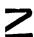
\includegraphics[keepaspectratio]{images/part001_a9d92cc3.jpg}}

显然 n 包含该表示的核。当 M 半单时（命题 4 (c)），n 等于该核，但一般并非如此。应注意，g 中满足 \(x_{M}\) 幂零的元素 x 不一定属于 n。

还要指出，引理 3 的一个特殊情形立即给出以下结果：

命题 5。设 \(\mathbf{V}\) 是 \(n\) 上维数为 \(\mathbf{K}\) 的向量空间，\(g\) 是 \(\mathfrak{gl}(\mathbf{V})\) 的李子代数，且其元素都是 \(\mathbf{V}\) 的幂零自同态。则存在递降的向量子空间序列 \(\mathrm{V}_0, \mathrm{V}_1, \ldots, \mathrm{V}_n\)（其均为 \(\mathbf{V}\) 的子空间），维数为 \(n, n - 1, \ldots, 0\)，使得 \(x(\mathrm{V}_i) \subset \mathrm{V}_{i+1}\) 对所有 \(x \in g\) 及 \(i = 0, 1, \ldots, n - 1\) 成立。

